\section{Conclusions}

\frame
{
	\frametitle{Synth\`ese}
	
	\begin{itemize}
		\item Norme incontournable.
		\item<2-> Adopt\'e par la majorit\'e des acteurs (constructeurs, \'editeurs de logiciels, clients).
		\item<3-> Spectre plus large que l'imagerie radiologique.
		\item<4-> Conseil : pr\'evoir DICOM d\`es l'achat de l'\'equipement.
		\begin{itemize}
			\item<5-> M\^eme si l'export des images se fera plus tard.
			\item<6-> Surco\^ut restera inf\'erieur \`a l'achat d'options a posteriori.
		\end{itemize}
		\item<7-> S'ouvrir aux autres standards et normes.
		\item<8-> Se mettre \`a jour. 
		\item<9-> Pr\'evoir plut\^ot que subir !
	\end{itemize}
}

\frame
{
    \frametitle{Exercice}
    Trouver les erreurs dans les m\'etadonn\'ees suivantes, en fonction du tableau fourni.
    En d\'eduire les cas qui seront rejet\'es par votre PACS.

	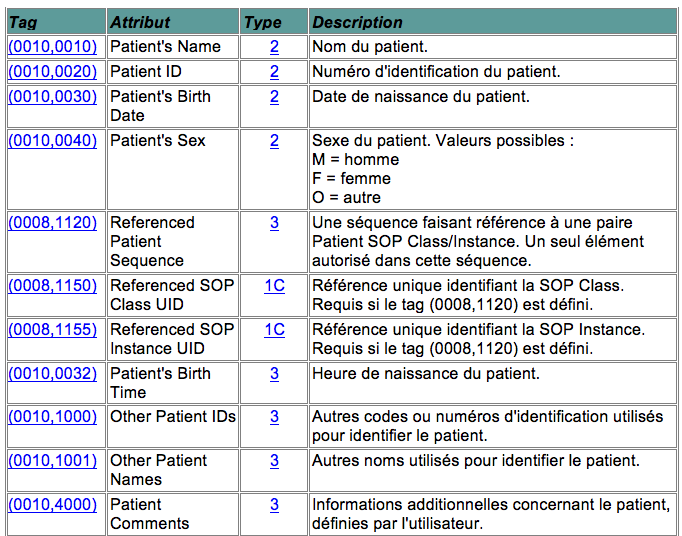
\includegraphics[width=.48\linewidth]{./figures/table.png}
	\hfill
	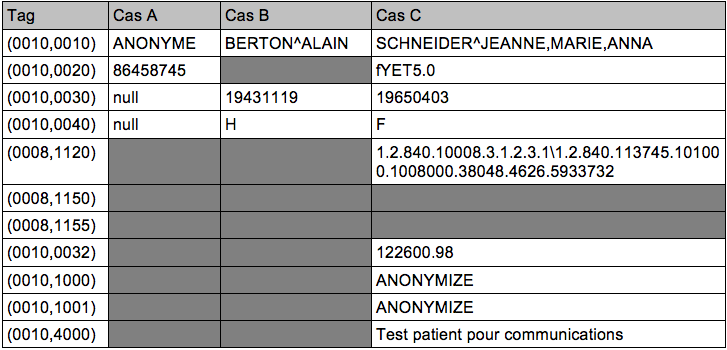
\includegraphics[width=.48\linewidth]{./figures/metadata-cases.png}
    
    Les cases gris\'ees indiquent un champ absent, \emph{null} un champ pr\'esent, mais vide.
}

